\section{Correlation of data}

One way to detect exoplanets in a time series, such as the one being analysed here, is to use an auto-correlatin function. This is possible because the decrease in luminousity caused by the exoplanet passing in front of the star will happen with a set periode (the periode of the exoplanets orbit). It is therefore expected that theese dips wil show up in the correlation as lags where the fit is better than usual. In order to get a usable result the timeseries has to be `flattened', removing the features caused by the drift in the telescope calibration. This is done by using a moving mean filter with a binsize of 50 (chosen to be big enough that the interesting features are not removed, while still being small enough to remove all the unwanted features) and subtracting this from the raw data, leaving only the flat data. \\

\begin{figure}[h]
\centering
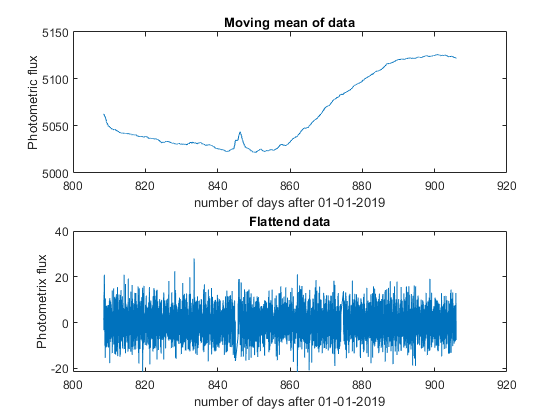
\includegraphics[width=\textwidth]{matlabstuff/flat_data.png}
\caption{Moving mean and flattened dataseries}%
\label{fig:flatData}
\end{figure}

The flattened data and the moving mean are shown in \autoref{fig:flatData}.\\

\begin{figure}[h]
\centering
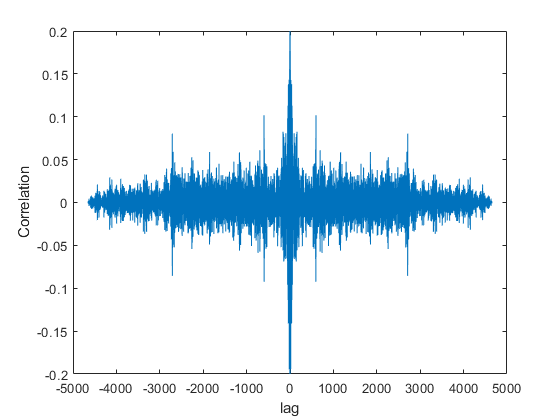
\includegraphics[width=\textwidth]{matlabstuff/Kepler_autoCorr.png}
\caption{Autocorrelation of time series}%
\label{fig:autoCorr}
\end{figure}

It is now possible to autocorrelate the data to see if there are any periodic behaviour. This is shown in \autoref{fig:autoCorr}. The center peak is of cource the complete overlap of the data, and goes up to one. It is also clear that there is a handfull of lags with a decent overlap. The larges of these are suspected to be the gaps in the data linig up. There are a series of smaller peaks which appear somewhat evenly spaced out, at around 400--450 steps. This could very well be an exoplanet, though it might also be some other feature of the star.

\begin{figure}[h]
\centering
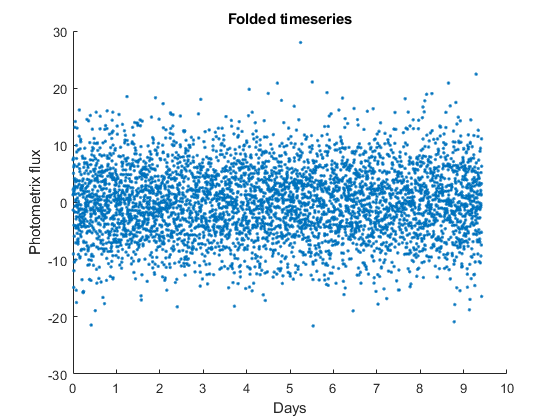
\includegraphics[width=\textwidth]{matlabstuff/fold_data.png}
\caption{Time series folded to match the possible exoplanet periode}%
\label{fig:foldData}
\end{figure}

One way to check if the feature is actually an exoplanet the timeseries if folded so the datapoints of the feature will overlap. This is shown in figure \autoref{fig:foldData}. It is clear from the figure that there is no significant feature in the data with the found frequency.\\
The star meassured is KIC10001893, which have the signs of three exoplanets\footnote{https://arxiv.org/abs/1409.6975}. The features might not, however, be actual planets after all\footnote{https://arxiv.org/abs/1906.03321}. Given the questionable nature of the exoplanets surrounding KIC10001893, it is not surprising that they are not found using the relatively simple autocorrelation.
